\documentclass[11pt]{article}
\usepackage[T1]{fontenc}
\usepackage{lmodern,amsmath,booktabs,graphicx}
\usepackage[margin=1in]{geometry}
\usepackage[colorlinks=true,linkcolor=blue,citecolor=blue,urlcolor=blue]{hyperref}
\hypersetup{pdfauthor={Qianghao Wu},pdftitle={The reported lunar-phase signal in US precipitation: a held-out test and a null that keeps spatial correlation}}
\title{The reported lunar-phase signal in US precipitation:\\ a held-out test and a null that keeps spatial correlation}
\author{Qianghao Wu}
\date{November 25, 2026}
\newcommand{\Rtwo}{R^2_2}
\begin{document}
\maketitle
\begin{abstract}
Cerveny, Svoma and Vose (2010) reported that, at 1218 US Historical Climatology Network (HCN) stations in 1895--2008, the second harmonic of the lunar synodic month explains 0.4106 of the variance of national mean daily precipitation in 10 lunar-phase classes ($p<0.03$), and that 23.1\% of the stations have a significant second harmonic. We pre-registered a test of both statistics on held-out GHCN-Daily data for 2009--2026. The null model rotates the lunar phase by a random amount in each calendar year, at all stations together, so it keeps the correlation between stations. In the held-out years neither statistic is significant (national $\Rtwo=0.40$, $p=0.41$; station rate 5.2\%, $p=0.57$). These 18 years detect a lunar modulation of precipitation of 10\% with power 0.97 or more and one of 5\% with power 0.36 to 0.52. They cannot detect one of about 1\%. In 1895--2008 we reproduce the national statistic ($\Rtwo=0.49$, first maximum 4.5 days after new moon), but it is not significant under the same null ($p=0.12$) or under an $F$ test ($p=0.09$). With the pre-registered station test, 8.05\% of the stations are significant (null mean 5.5\%, $p=0.10$). A more liberal station test gives 23.4\%, close to the published 23.1\%, against a null mean of 17.8\%. In exploratory analyses, the 1895--2008 station rate is at the 0.05 boundary: its $p$-value goes from 0.02 to 0.14 with the hour of the phase computation, which the source does not state. With a null that keeps the correlation between stations, the data do not support the reported significance of the signal, and they cannot exclude an effect of about 1\%.

This work has not yet been reviewed by experts. The computations, the proofs and the text were produced by AI models (from Anthropic and OpenAI), working under the author's direction.
\end{abstract}
\medskip
\noindent\textit{Keywords:} lunar synodic month, precipitation, Historical Climatology Network, GHCN-Daily, field significance, pre-registration, placebo test

\section{Introduction}
Bradley, Woodbury and Brier (1962) reported that heavy precipitation at 1544 US stations in 1900--1949 was more frequent in the first and third weeks of the lunar synodic month~\cite{bradley1962}. Brier and Bradley (1964) found a 14.765-day wave, half of the 29.53-day synodic month, in these data. They split 1900--1949 into two 25-year halves and found the same phase in both~\cite{brier1964}. Lund (1965) found a similar period in US sunshine records. As summarized by Camuffo, Lund warned that ``the possibility that its appearance is due to a combination of the smoothing procedure and the temporal and spatial correlation among the observations cannot be ignored''~\cite{lund1965,camuffo2001}. Hanson, Maul and McLeish (1987) found that the phase of the lunar precipitation relation moves across the United States~\cite{hanson1987}.

Cerveny, Svoma and Vose (2010) returned to the question with the HCN daily precipitation of 1218 stations for 1895--2008~\cite{cerveny2010}. They standardized each station's daily values and put each day in one of 10 lunar-phase classes. They state (paragraphs [12] and [13]):

\begin{quote}
``When harmonic analysis is applied to the lunar-categorized data, the variance explained by the second harmonic is 0.4106 ($p<0.03$).'' [\dots] ``A large number (281, or 23.1 percent of all stations) of HCN precipitation stations---again some as far inland as the upper Midwest---display explained variances by a second-order harmonic for the synodic month period which are statistically significant at the 0.05 confidence level.''
\end{quote}

The first maximum of the national second harmonic is 4.04 days after new moon. The paper used this signal to explain a lunar signal in US streamflow.

Two points of the source are open. First, the paper does not state its significance tests. With 10 class means and a two-parameter harmonic, an $F(2,7)$ test of $r^2=0.4106$ gives $p=0.157$, not $p<0.03$. Second, the station rate counts 1218 stations as if they were independent. Nearby stations share the same storms, so a single wet day near a given phase moves many stations at the same time. For its streamflow tests, the paper itself notes that the tests ``require independence of observations (likely not the case for the streamflow data due to spatial autocorrelation)'' and adds a Monte Carlo test~\cite[para.~5]{cerveny2010}. It applies no such correction to the precipitation station rate. This is the problem of field significance~\cite{livezey1983}.

We searched the citing literature, arXiv, Zenodo, GitHub and the web for a re-test of the 2010 precipitation claim (Section~\ref{sec:prior}). We found none. This paper gives three things:
\begin{enumerate}
\item a pre-registered test of both statistics on 2009--2026, data that did not exist in 2010;
\item a null model that keeps the correlation between stations and between days, applied to 1895--2008 and to 2009--2026;
\item placebo periods and injected signals of known size, which show what the test can and cannot detect.
\end{enumerate}

\begin{quote}
\textbf{The claim does not replicate in 2009--2026, but these years cannot detect an effect of about 1\%. In 1895--2008 the national harmonic is not significant once the null keeps the spatial correlation. The 1895--2008 station rate is at the 0.05 boundary, and its $p$-value depends on the hour of the phase computation.}
\end{quote}

\section{Data and pre-registration}
\paragraph{Data.} We used the HCN subset of NOAA NCEI GHCN-Daily~\cite{menne2012}, file \texttt{ghcnd\_hcn.tar.gz}, version 3.35-upd-2026111517 (316,596,781 bytes, SHA-256 \texttt{b327e62d\dots a2151}). We kept the element \texttt{PRCP} at the 1218 stations of the archive in the conterminous US. A value is valid if it is not missing and its quality flag is blank. The lunar phase comes from the JPL ephemeris DE440s~\cite{park2021} through the Skyfield library~\cite{skyfield}.

\paragraph{Periods.} Period A (in-sample) is 1895-01-01 to 2008-12-31, the period of the source. Period B (held out) is 2009-01-01 to 2026-10-31. A station enters A with at least 3650 valid days in A, and B with at least 2000 valid days in B. A has 1217 stations and 41.0 million station-days. B has 980 stations and 5.5 million station-days. Each period has its own standardization and its own station list.

\paragraph{Pre-registration.} The test, the null, the controls and the decision rules were committed to the repository before any precipitation value was read (\texttt{PROTOCOL.md}, commit \texttt{783c7b0}). All later analyses are in dated addenda that state what we saw before each one. They are labelled exploratory here.

\section{Method}
\paragraph{Lunar phase.} The source computes the phase ``by determining the average angular difference between the apparent longitudes of the moon and sun for that day''~\cite[para.~11]{cerveny2010}. It does not give an hour. We pre-registered the elongation $E$ (apparent geocentric ecliptic longitude of the Moon minus that of the Sun, of date) at 12:00 UTC of the observation date. This is about 06:00 to 07:00 local standard time in the conterminous US. Brier and Bradley used Greenwich noon~\cite{brier1964}. Fine bins are $f=\lfloor E/3.6^\circ\rfloor$, $f=0,\dots,99$. Class $k=\lfloor f/10\rfloor+1$ runs from 1 to 10. Class 1 starts at new moon, and full moon is at the boundary of classes 5 and 6.

\paragraph{Statistic.} For each station and period, $z=(p-\bar p)/s$ over the valid days. The national class mean $m_k$ is the mean of $z$ over all station-days in class $k$. With class-centre angles $\theta_k=2\pi(k-0.5)/10$,
\[
a_2=\tfrac{2}{10}\sum_k m_k\cos 2\theta_k,\quad b_2=\tfrac{2}{10}\sum_k m_k\sin 2\theta_k,\quad
\Rtwo=\frac{5(a_2^2+b_2^2)}{\sum_k (m_k-\bar m)^2}.
\]
The first maximum is at $\tfrac12\operatorname{atan2}(b_2,a_2)\bmod\pi$, converted to days with 29.530589 days per cycle. The station test computes the same $\Rtwo$ from the 10 class means of one station. The station is significant if $F=(\Rtwo/2)/((1-\Rtwo)/7)$ gives $p<0.05$ with $(2,7)$ degrees of freedom. The station rate $S$ is the share of significant stations.

\paragraph{Null model: year-wise random rotation (YRR).} In each replicate, each calendar year gets one random integer offset $u\in\{0,\dots,99\}$, independent between years. Every day of that year, at every station, gets the fine bin $(f+u)\bmod 100$. The rotation keeps all correlation between stations and all correlation inside a year. It removes any fixed relation to the true phase. We used 2000 replicates and $p=(1+\#\{\text{null}\ge\text{observed}\})/2001$.

\paragraph{Decision rules (period B).} H1: the national $\Rtwo$ has YRR $p<0.05$ and its first maximum is within $\pm3.69$ days of 4.04 days. H2: the station rate $S$ has YRR $p<0.05$. If neither holds, the claim fails to replicate. That verdict counts against an effect of the 1895--2008 size only if injected signals of that size are detected in B with power at least 0.8.

\paragraph{Controls.} (i) Placebo phases: a pseudo-phase with a fixed period $P$, for $P=27.3$, 28.5, 30.5 and 31.0 days, and for a scan from 25.00 to 35.00 days in steps of 0.05 days. The lunar value counts as distinct if it exceeds the 95th percentile of the 161 scan periods more than 1 day from 29.53 days. (ii) Known-answer injection: raw precipitation becomes $p'=p\,(1+c\cos(2\theta-\varphi_0))$ with its first maximum at 4.04 days, for $c$ from 0 to 0.10, with 200 draws per $c$ on YRR-rotated phases.

\section{Results}
\subsection{Held-out period, 2009--2026 (pre-registered decision)}
The national $\Rtwo$ in B is 0.399, with YRR $p=0.41$. The first maximum is 3.23 days after new moon. This is inside the window of H1, but half of all random phases are inside that window. H1 is not met. The station rate is $S=51/980=5.2\%$, with YRR $p=0.57$. H2 is not met. The verdict is ``fails to replicate''.

The power condition is not met. The observed period-A amplitude corresponds to an injected modulation of $c\approx0.0096$, about 1\%. At this size, B detects the national signal with power 0.05 and the station signal with power 0.045. B detects $c=0.10$ with power 0.985 (national) and 0.97 (stations), and $c=0.05$ with power 0.52 and 0.355 (Table~\ref{tab:inj}). So the held-out result is underpowered. It does not by itself refute an effect of the 1895--2008 size.

\begin{figure}[t]
\centering
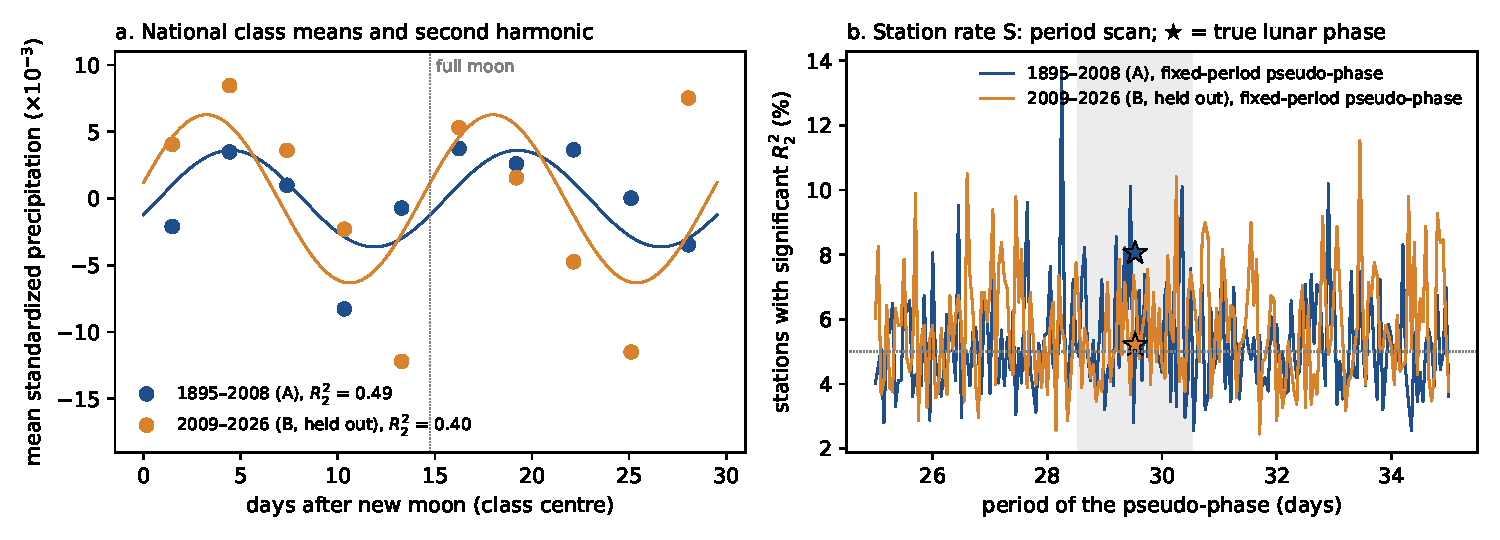
\includegraphics[width=\textwidth]{figures/fig1.pdf}
\caption{(a) National mean of standardized daily precipitation in the 10 lunar-phase classes, with the fitted mean plus second harmonic, for 1895--2008 and for the held-out 2009--2026. (b) Station rate $S$ (pre-registered $F$ test) when the lunar phase is replaced by a pseudo-phase of fixed period $P$. Stars: the true lunar elongation. Grey band: periods within 1 day of 29.53 days, left out of the placebo distribution. Dotted line: the nominal 5\% rate for independent stations.}
\label{fig:main}
\end{figure}

\subsection{In-sample period, 1895--2008}
\begin{table}[h]
\centering
\small
\begin{tabular}{lcc}
\toprule
Period A, 1895--2008 & Source~\cite{cerveny2010} & This study\\
\midrule
Stations & 1218 & 1217\\
National $\Rtwo$ of the 10 class means & 0.4106 & 0.494\\
First maximum after new moon & 4.04 d & 4.49 d\\
$p$, $F(2,7)$ on the 10 means & --- & 0.092\\
$p$, YRR null & $<0.03$ (test not stated) & 0.124\\
Station rate $S$, $F(2,7)$ station test & 23.1\% (281) & 8.05\% (98)\\
$p$ of $S$, YRR null (null mean 5.5\%, 95th percentile 9.0\%) & --- & 0.099\\
$p$ of $S$, binomial, stations treated as independent & --- & $3.9\times10^{-6}$\\
\bottomrule
\end{tabular}
\caption{Reproduction in 1895--2008 with the pre-registered 12:00 UTC phase.}
\label{tab:A}
\end{table}

The national statistic is close to the published one by the pre-registered rule ($|\Rtwo-0.4106|\le0.15$ and phase within $\pm1.5$ days). Figure~\ref{fig:main}a shows the class means. The national statistic is not significant under the $F$ test ($p=0.092$) or under the YRR null ($p=0.124$).

The pre-registered station rate is 8.05\%. If the stations were independent, this rate would have $p=3.9\times10^{-6}$. Under the YRR null, which keeps the shared weather, its $p$ is 0.099. Two other runs with independent sets of 2000 replicates gave 0.088 and 0.084. The YRR null distribution of $S$ is wide because nearby stations share the same storms. This is Lund's point, now measured on the 2010 statistic.

\paragraph{Placebo periods.} Table~\ref{tab:placebo} gives the four fixed placebo periods. In the scan of period A, 15 of the 161 far periods give a higher national $\Rtwo$ than the lunar phase. The lunar $\Rtwo$ is not distinct. For the station rate, 6 of 161 far periods are higher, so the lunar $S$ is distinct by the pre-registered rule (95th percentile 7.5\%). The highest placebo $S$ is 13.7\% at 28.25 days (Figure~\ref{fig:main}b). In period B neither statistic is distinct (40 and 94 of 161 far periods are higher).

\begin{table}[h]
\centering
\begin{tabular}{lcccc}
\toprule
Period (days) & A: $\Rtwo$ & A: $S$ & B: $\Rtwo$ & B: $S$\\
\midrule
27.3 & 0.139 & 5.4\% & 0.193 & 6.9\%\\
28.5 & 0.115 & 5.2\% & 0.063 & 7.8\%\\
29.530589 (mean synodic month) & 0.525 & 8.3\% & 0.406 & 5.9\%\\
30.5 & 0.660 & 7.6\% & 0.092 & 7.4\%\\
31.0 & 0.277 & 5.8\% & 0.041 & 4.7\%\\
True lunar elongation & 0.494 & 8.05\% & 0.399 & 5.2\%\\
\bottomrule
\end{tabular}
\caption{National $\Rtwo$ and station rate $S$ for fixed-period pseudo-phases.}
\label{tab:placebo}
\end{table}

\paragraph{Injections.} Table~\ref{tab:inj} gives the power. At $c=0$ the rejection rates are 0.025 to 0.04. The injection draws and the null draws use the same rotation scheme, so this rate is near 0.05 by construction. It shows that the code is consistent. It does not show that the YRR null is valid for real data. An independent verifier used a second null that permutes whole years, and it gave the same conclusions. In A, a 3\% lunar modulation would be detected with power 0.87. The observed A amplitude (0.00362) is equal to the mean injected amplitude at $c\approx0.0096$. Noise alone gives a mean amplitude of 0.00244, and the observed amplitude is inside the null range. So $c\approx1\%$ is an upper estimate of a true effect. The true effect can be zero.

\begin{table}[h]
\centering
\begin{tabular}{lcccc}
\toprule
$c$ & A: national & A: $S$ & B: national & B: $S$\\
\midrule
0 & 0.03 & 0.04 & 0.025 & 0.04\\
0.005 & 0.08 & 0.05 & 0.04 & 0.045\\
0.01 & 0.185 & 0.075 & 0.05 & 0.045\\
0.02 & 0.58 & 0.34 & 0.095 & 0.06\\
0.03 & 0.87 & 0.745 & 0.205 & 0.115\\
0.05 & 1.0 & 1.0 & 0.52 & 0.355\\
0.10 & 1.0 & 1.0 & 0.985 & 0.97\\
\bottomrule
\end{tabular}
\caption{Power at YRR level 0.05 for an injected multiplicative modulation of size $c$ (200 draws per value; national power includes the phase condition of H1).}
\label{tab:inj}
\end{table}

\subsection{Exploratory analyses}
The analyses in this section were added after we saw the primary results. They are not pre-registered. The protocol addenda record what we saw before each one. We do not correct them for the full number of exploratory comparisons.

\paragraph{The published 23.1\% matches a liberal station test.} If a station counts as significant when a two-sided $t$ test of $r=\sqrt{\Rtwo}$ with 8 degrees of freedom gives $p<0.05$ (that is, $\Rtwo>0.399$), the period-A station rate is $285/1217=23.4\%$. The source reports $281/1218=23.1\%$. This test treats the two-parameter harmonic as a one-parameter correlation. Under independent noise ($\Rtwo\sim\mathrm{Beta}(1,3.5)$) it flags 16.8\% of stations. Under the YRR null its mean rate is 17.8\% (95th percentile 24.8\%), and the observed 23.4\% has $p=0.092$. In B the same test gives 20.4\% ($p=0.25$). The one-sided version of this $t$ test gives $p=0.023$ for the published national $\Rtwo=0.4106$, which matches the published ``$p<0.03$''. It is not confirmed that the source used these tests. The source does not state its tests, and the match of 23.4\% with 23.1\% is the only evidence.

\paragraph{Pooled period.} On 1895-01 to 2026-10 together (1218 stations; 87.9\% of the station-days are from A), the national $\Rtwo$ is 0.641 with first maximum at 4.24 days and YRR $p=0.049$. The station rate is $105/1218=8.6\%$ with YRR $p=0.055$ (null mean 5.4\%). These values are near the 0.05 boundary. Most of the pooled data are from period A, so they are not independent of the period-A results. An independent implementation that used a 13-term series for the lunar elongation got 111 stations. That series puts 20 of 48,152 days in another class. With the same code and the DE440s elongation the count is 105. The station count changes with very small changes of the phase, because many stations are near the threshold.

\paragraph{Timing of the phase.} The source gives the phase ``for that day'' with no hour~\cite[para.~11]{cerveny2010}. GHCN-Daily dates can also lag the true rain day by one day at stations that read the gauge in the morning. An independent verifier therefore computed the phase at five times for each observation date $d$. We repeated this with our own code (protocol addendum 3). Table~\ref{tab:timing} gives the results. ``Adjusted'' is the $p$-value of the smallest of the five $p$-values against the null distribution of that smallest $p$-value. \emph{The adjustment corrects only for the choice among the five timings. It does not correct for the other post hoc choices: two station tests, three periods, and the national against the station statistic.}

\begin{table}[h]
\centering
\small
\begin{tabular}{llcccccc}
\toprule
Period & Timing & $\Rtwo$ & $p$ & Stations, $F$ & $p$ & Stations, two-sided $t$ & $p$\\
\midrule
A & 12 UTC, $d$ (protocol) & 0.494 & 0.116 & 98 & 0.084 & 285 & 0.071 \\
A & 00 UTC, $d$ & 0.519 & 0.096 & 100 & 0.067 & 290 & 0.060 \\
A & 18 UTC, $d$ & 0.540 & 0.081 & 118 & 0.023 & 299 & 0.052 \\
A & 12 UTC, $d-1$ & 0.475 & 0.126 & 88 & 0.136 & 310 & 0.033 \\
A & 12 UTC, $d+1$ & 0.480 & 0.128 & 122 & 0.020 & 333 & 0.018 \\
A & adjusted for 5 timings & & 0.156 & & 0.038 & & 0.033 \\ \midrule
B & 12 UTC, $d$ (protocol) & 0.399 & 0.402 & 51 & 0.568 & 200 & 0.260 \\
B & 00 UTC, $d$ & 0.576 & 0.195 & 54 & 0.503 & 174 & 0.540 \\
B & 18 UTC, $d$ & 0.501 & 0.281 & 58 & 0.403 & 184 & 0.405 \\
B & 12 UTC, $d-1$ & 0.417 & 0.374 & 34 & 0.934 & 175 & 0.508 \\
B & 12 UTC, $d+1$ & 0.548 & 0.220 & 38 & 0.866 & 164 & 0.639 \\
B & adjusted for 5 timings & & 0.340 & & 0.620 & & 0.428 \\ \midrule
Pooled & 12 UTC, $d$ (protocol) & 0.641 & 0.043 & 105 & 0.056 & 303 & 0.053 \\
Pooled & 00 UTC, $d$ & 0.663 & 0.034 & 106 & 0.057 & 290 & 0.074 \\
Pooled & 18 UTC, $d$ & 0.660 & 0.035 & 118 & 0.026 & 310 & 0.036 \\
Pooled & 12 UTC, $d-1$ & 0.633 & 0.050 & 89 & 0.149 & 300 & 0.053 \\
Pooled & 12 UTC, $d+1$ & 0.634 & 0.046 & 140 & 0.007 & 350 & 0.008 \\
Pooled & adjusted for 5 timings & & 0.078 & & 0.015 & & 0.018 \\
\bottomrule
\end{tabular}
\caption{Timing sensitivity (exploratory). YRR $p$-values from 2000 replicates (seed 20261125), one rotation per replicate for all five timings. Stations in A, B and pooled: 1217, 980 and 1218. 18:00 UTC is about local noon in the conterminous US. The adjusted $p$-values correct only for the choice among the five timings.}
\label{tab:timing}
\end{table}

The findings are:
\begin{itemize}
\item Period B shows no signal for any timing. The smallest $p$ is 0.195.
\item The period-A national $\Rtwo$ is not significant for any timing ($p$ from 0.08 to 0.13; adjusted 0.156).
\item The period-A station rate ($F$ test) has $p$ from 0.020 to 0.136. Two of the five timings give $p<0.05$. The adjusted $p$ is 0.038, and it corrects only for the timing choice. With the two-sided $t$ test the adjusted $p$ is 0.033, with the same restriction.
\item The pooled station rate has adjusted $p=0.015$ ($F$ test) and 0.018 ($t$ test), again corrected only for the timing choice. The pooled national $\Rtwo$ has adjusted $p=0.078$.
\end{itemize}
The 12 UTC $p$-values of this table differ a little from Table~\ref{tab:A} (0.116 against 0.124; 0.084 against 0.099) because the random seed is different. This is Monte Carlo error.

\section{Interpretation}
\begin{itemize}
\item Computed: with the statistic of the source, 1895--2008 HCN data give a national second harmonic close to the published one ($\Rtwo=0.49$, first maximum 4.5 days after new moon).
\item Computed: that national harmonic is not significant at 0.05 once the null keeps the correlation between stations and between days. This holds for each of the five timings of the phase. In the scan from 25 to 35 days, 15 of the 161 placebo periods give a larger national $\Rtwo$.
\item Computed: the 1895--2008 station rate is at the 0.05 boundary under the same null. It is exploratory. Its $p$-value depends on the hour of the phase (0.02 to 0.14 over five timings). In the period-A scan, the lunar station rate is distinct by the pre-registered placebo rule (6 of 161 far periods are higher). Most of the published 23.1\% is expected with no lunar effect: the liberal test that reproduces it has a null mean of 17.8\%.
\item Not proved: a weak lunar-phase association in the 1895--2008 station rates. The evidence for it depends on post hoc choices, and the held-out period does not show it.
\item Computed: 2009--2026 shows no signal. These 18 years detect a modulation of 10\% with power 0.97 or more and one of 5\% with power 0.36 to 0.52. They cannot detect one of about 1\%.
\item Believed, not proved: a lunar modulation of about 1\%, if it exists, cannot be separated from weather noise in the HCN record. We do not claim that the lunar effect is zero.
\end{itemize}

\section{How the result was checked}
\begin{itemize}
\item The script \texttt{checks/rerun.py} downloads the raw public data, recomputes every number in this paper, and compares 252 values with \texttt{data/expected.json}. The tolerances are, for example, $\pm0.01$ on $\Rtwo$, $\pm3$ on station counts and $\pm0.02$ on $p$-values.
\item An independent verifier, using a different AI model, wrote three implementations that import nothing from our code: its own archive parser, its own lunar phase (a Meeus series in the first one, a separate Skyfield call in the second and third), and a direct YRR null. The parsed precipitation array was equal to ours in every cell. All observed values agreed. The $p$-values agreed within Monte Carlo error. A null that permutes whole years gave the same conclusions. The third implementation, with another random seed, confirmed the timing table for periods A and B (period-A station rate, adjusted $p$ 0.041 against our 0.038). Its run for the pooled period did not finish.
\item The verifier also checked the source quote three times against the published text, and checked in the git history that the protocol and each addendum were committed before their outcome files.
\item The numbers of this paper are from GHCN-Daily version 3.35-upd-2026111517. On 2026-11-25 the verifier reran \texttt{checks/rerun.py} from a clean clone with fresh downloads. NCEI had updated the archive to version 3.35-upd-2026112318 (316,612,378 bytes, SHA-256 \texttt{2f94aed8}\allowbreak\texttt{5c4fc0b9}\allowbreak\texttt{967c95ca}\allowbreak\texttt{b87490c0}\allowbreak\texttt{9d0e6fd0}\allowbreak\texttt{0baa2414}\allowbreak\texttt{7b70fd66}\allowbreak\texttt{40a81148}). The result was 252 of 252 values inside the tolerances. 46 values were not bit-equal, all in period B or the pooled period. The largest changes were the placebo $S$ at 31.0 days in B (4.69\% to 4.59\%) and the B national $\Rtwo$ (0.39925 to 0.39934). The verdict was the same.
\end{itemize}

\section{Limits}
\begin{itemize}
\item NCEI updates GHCN-Daily every day and does not keep old versions at the same URL. A later download can differ a little, and after enough updates some values can leave the tolerances.
\item The current GHCN-Daily HCN values differ from the 2010 HCN daily files (later quality control, added data). Our period A has 1217 stations, the source 1218.
\item The source does not give the hour of its phase or its tests. We pre-registered 12:00 UTC of the observation date. Table~\ref{tab:timing} shows that the national $\Rtwo$ and the period-B result do not depend on this choice, but the period-A and pooled station rates do.
\item The YRR null uses calendar years as blocks. It keeps correlation inside a year and between all stations. It does not keep year-to-year persistence that is tied to the lunar phase.
\item Only precipitation was tested. Streamflow, the main topic of the source, was not tested.
\end{itemize}

\section{Prior work}\label{sec:prior}
We searched on 2026-11-24 and 2026-11-25: the papers that cite the source (22 records in Semantic Scholar, 20 in OpenAlex), later citers of Bradley et al.\ (1962) and Brier and Bradley (1964), the later papers of the source authors, arXiv, Zenodo, GitHub, a public collection of AI-produced research results, and web and semantic searches. Studies since 2010 examine other regions (Mexico, Pakistan, Sri Lanka, Israel), other variables (semidiurnal river tides, circulation, lunar declination) or other time scales. We found no re-test of the 2010 US precipitation claim with held-out years, placebo periods or a null that keeps spatial correlation. The nearest earlier checks are in Brier and Bradley~\cite{brier1964}: a split-half test of 1900--1949 and a check on independent data (a daily US precipitation index for 1950--1959, and four stations from 1871). These checks test their own claim, on older data and with different statistics.

\paragraph{Reproduction.} Run \texttt{bash checks/ci.sh} from the result folder. It installs pinned packages, downloads about 350 MB, recomputes the study and compares 252 values. The source code, the protocol and the verification reports accompany this paper.

\begin{thebibliography}{10}
\bibitem{bradley1962} D. A. Bradley, M. A. Woodbury and G. W. Brier, ``Lunar synodical period and widespread precipitation,'' \emph{Science} 137, 748--749 (1962). \href{https://doi.org/10.1126/science.137.3532.748}{doi:10.1126/science.137.3532.748}.
\bibitem{brier1964} G. W. Brier and D. A. Bradley, ``The lunar synodical period and precipitation in the United States,'' \emph{J. Atmos. Sci.} 21, 386--395 (1964). \href{https://doi.org/10.1175/1520-0469(1964)021<0386:TLSPAP>2.0.CO;2}{doi:10.1175/1520-0469(1964)021$<$0386:TLSPAP$>$2.0.CO;2}.
\bibitem{lund1965} I. A. Lund, ``Indications of a lunar synodical period in United States observations of sunshine,'' \emph{J. Atmos. Sci.} 22(1), 24--39 (1965). \href{https://doi.org/10.1175/1520-0469(1965)022<0024:IOALSP>2.0.CO;2}{doi:10.1175/1520-0469(1965)022$<$0024:IOALSP$>$2.0.CO;2}. Cited here as summarized in~\cite{camuffo2001}.
\bibitem{camuffo2001} D. Camuffo, ``Lunar influences on climate,'' \emph{Earth, Moon, and Planets} 85--86, 99--113 (1999). \href{https://doi.org/10.1023/A:1017099427908}{doi:10.1023/A:1017099427908}.
\bibitem{hanson1987} K. Hanson, G. A. Maul and W. McLeish, ``Precipitation and the lunar synodic cycle: phase progression across the United States,'' \emph{J. Climate Appl. Meteor.} 26, 1358--1362 (1987). \href{https://doi.org/10.1175/1520-0450(1987)026<1358:PATLSC>2.0.CO;2}{doi:10.1175/1520-0450(1987)026$<$1358:PATLSC$>$2.0.CO;2}.
\bibitem{cerveny2010} R. S. Cerveny, B. M. Svoma and R. S. Vose, ``Lunar tidal influence on inland river streamflow across the conterminous United States,'' \emph{Geophys. Res. Lett.} 37, L22406 (2010). \href{https://doi.org/10.1029/2010GL045564}{doi:10.1029/2010GL045564}.
\bibitem{livezey1983} R. E. Livezey and W. Y. Chen, ``Statistical field significance and its determination by Monte Carlo techniques,'' \emph{Mon. Wea. Rev.} 111, 46--59 (1983). \href{https://doi.org/10.1175/1520-0493(1983)111<0046:SFSAID>2.0.CO;2}{doi:10.1175/1520-0493(1983)111$<$0046:SFSAID$>$2.0.CO;2}.
\bibitem{menne2012} M. J. Menne, I. Durre, R. S. Vose, B. E. Gleason and T. G. Houston, ``An overview of the Global Historical Climatology Network-Daily database,'' \emph{J. Atmos. Oceanic Technol.} 29, 897--910 (2012). \href{https://doi.org/10.1175/JTECH-D-11-00103.1}{doi:10.1175/JTECH-D-11-00103.1}. Data: \url{https://www.ncei.noaa.gov/pub/data/ghcn/daily/}.
\bibitem{park2021} R. S. Park, W. M. Folkner, J. G. Williams and D. H. Boggs, ``The JPL planetary and lunar ephemerides DE440 and DE441,'' \emph{Astron. J.} 161, 105 (2021). \href{https://doi.org/10.3847/1538-3881/abd414}{doi:10.3847/1538-3881/abd414}.
\bibitem{skyfield} B. Rhodes, Skyfield, version 1.55, \url{https://pypi.org/project/skyfield/}.
\end{thebibliography}
\end{document}
